\chapter{Architectural Design}
\labch{options}
	\section{Overview}
		From an implementation perspective, it was decided to develop the S\&C platform as a web application.For this reason, the architecture chosen for its development is a 3-tier architecture. It is a software design pattern that separates applications into three distinct layers:
		\begin{enumerate}
			\item \textbf{Presentation Layer}: The user interface (UI) where users interact with the application
			\item \textbf{Application Layer}: the layer in which the data are processed
			\item \textbf{Data Layer}: manages the storage, retrieval, and manipulation of data, involving databases
		\end{enumerate}
		
		This architecture offers significant advantages in terms of scalability, maintainability, and especially modularity, allowing each layer to be developed and updated independently of the others.
		
		Going into detail, the data layer employs two different types of databases: a relational database is used to manage the structured data of our system, which constitutes the majority of the data utilized by the platform (users, internship advice, internships, notifications, etc.). For the management of unstructured data, namely CVs and selection-related questionnaires, a non-relational database was chosen. Specifically, MongoDB was selected, as its JSON-based data storage format is perfectly suited for hierarchical and non-rigid structures, such as CVs and questionnaires.
		
		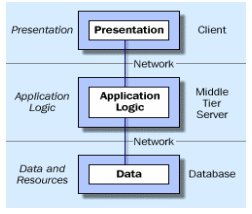
\includegraphics{3Tier.jpg}
		
		\section{Component View}
			As mentioned, the platform is developed used a 3-tier architecture approach with 2 DB(a RDBMS and MongoDB); As for the back-end components, four main macro-components can be identified, which are:
			\begin{enumerate}
				\item \textbf{Social Application System}: It provides the "social" functionalities of the platform, such as user registration/login, searching for internship advice, viewing profiles, applying for/sending an application proposal, sending feedback/complaints, and so on. It is divided in several components:
				\begin{enumerate}
					\item \textbf{Authentication Manager}: It handles user authentication (initial registration, subsequent logins);
					\item \textbf{Application Manager}: It is responsible for managing application proposals, acceptances, and application requests;
					\item \textbf{Advice Presenter}: It provides functionalities for viewing individual internship advice and the list of all internship advice published on the platform;
					\item \textbf{Advice Publisher}: It provides functionalities for publishing and deleting an internship advice;
					\item \textbf{Feedback Manager}: It provides functionalities for viewing feedback questionnaires and receiving the corresponding responses;
					\item \textbf{Internship Manager}: It displays the ongoing internships (both the list and individual ones) and manages user complaints;
					\item \textbf{Profile Manager}: it provides functionalities for managing a profile, from creation to modification and deletion
					\item \textbf{Profile Presenter}: It allows viewing profiles
					\end{enumerate}
					
					\item \textbf{Recommendation System}: It is the component responsible for the recommendation functionality offered by the platform, which involves analyzing the necessary information (feedback, CVs for students, etc.), determining which internships/students may be of interest to a specific user, and finally sending this information to the interested user. It is divided into 3 sub-components:
					\begin{enumerate}
						\item \textbf{Recommendation Interface}: It is the component that retrieves the necessary information from the databases to develop the recommendation;
						\item \textbf{Recommendation Analyzer}: t is the component that performs the analysis on the information obtained from the recommendation interface (feedback, CVs, etc.);
						\item \textbf{Recommendation Presenter}: It inserts the recommendation results into the database and triggers the sending of notifications to inform that the recommendation has been made
					\end{enumerate}
					
					\item \textbf{Selection Management System}: 
					It provides functionalities related to the entire selection process, from its configuration to the sending of results. It is divided in 3 sub-components:
					\begin{enumerate}
						\item \textbf{SP Initializer}: It provides functionalities for configuring the selection process (dates, metrics, questionnaires, etc.);
						\item \textbf{SP Manager}: It manages the insertion of answers in the questionnaires and the subsequent finalization of the selection process
						\item \textbf{SP presenter}: It displays interview dates and the results of the selection process
					\end{enumerate}
					
					\item \textbf{Notification System}: 
					It is the component responsible for managing all notifications generated and sent by the system; it handles the creation, sending, and triggering of notifications with the mail service. It is divided in 2 sub-components:
					\begin{enumerate}
						\item \textbf{Notification presenter}: It allows viewing notifications (both individual ones and the list);
						\item \textbf{Notification Generator}: It is the component that generates a notification and triggers the sending of an email;
					\end{enumerate}
			\end{enumerate}
			
			there are other important components of the system:
			\begin{enumerate}
				\item \textbf{DBMS}: stores all the structured data of the platform
				\item \textbf {WebServer}: it is the component related to routing the incoming request to the appropriate internal component.
				\item \textbf{MongoDB API}: A programming interface that allows developers to interact with a MongoDB database through HTTP requests, using CRUD operations (Create, Read, Update, Delete) on data stored in a MongoDB database;
				\item \textbf{SES API}: Amazon Simple Email Service (SES) is an email sending and receiving service offered by Amazon Web Services (AWS). The SES API allows to easily integrate email sending functionality into applications/websites.
			
			\end{enumerate}
			
			for the front-end, there are 2 clients which interact with the back-end:
			\begin{enumerate}
				\item \textbf{WebClient}: the UI of the application; it interacts with the back-end through REST API, which is based on a set of principles and constraints that allow systems to communicate over the web using standard HTTP methods such as GET, POST, PUT, DELETE, etc.
				\item \textbf{Client Mail}: the client used to access and manage the mail; it communicates with the back-end (in particular with the Notification system) through SES API
			\end{enumerate}
			
			the component diagram is shown in the following figure:
			
			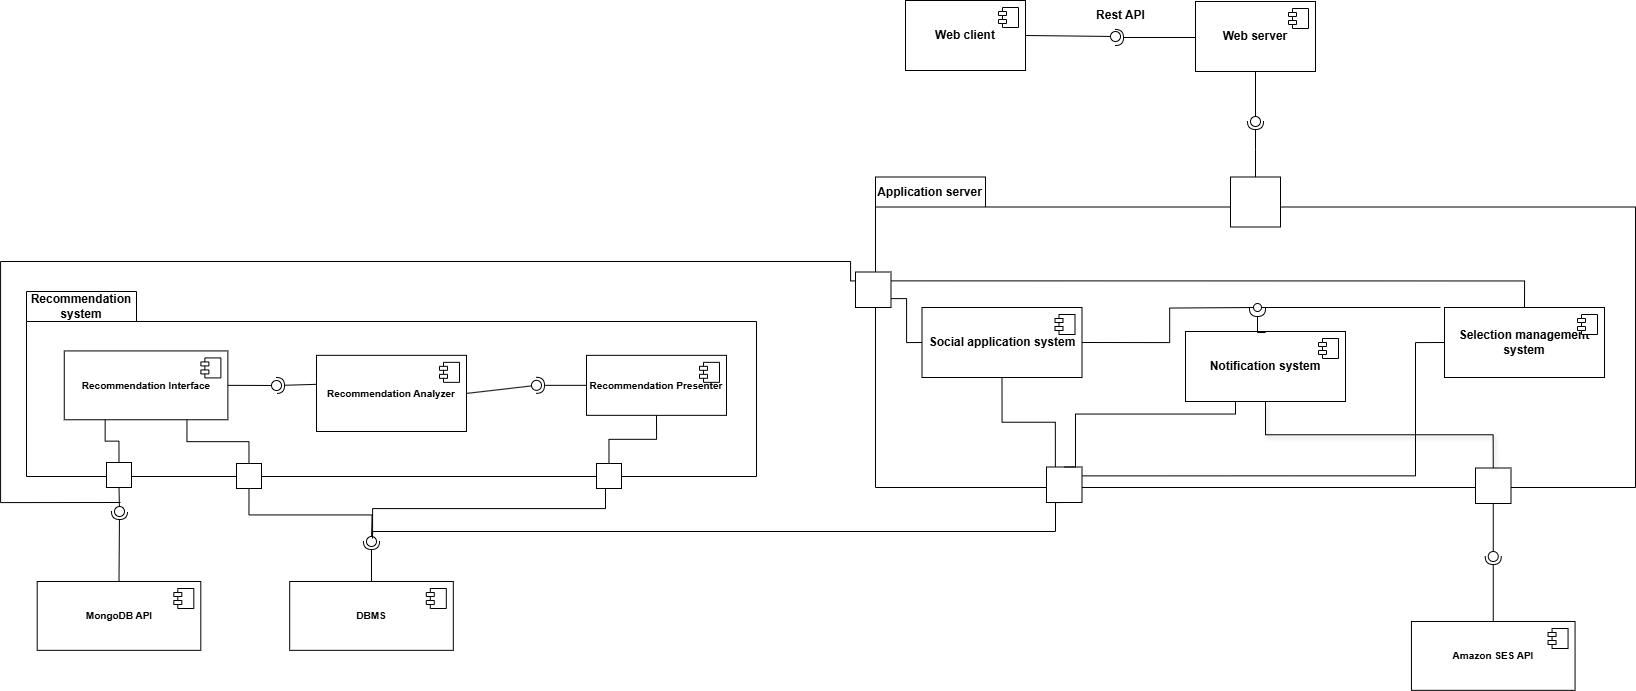
\includegraphics{componentView.png}
			
			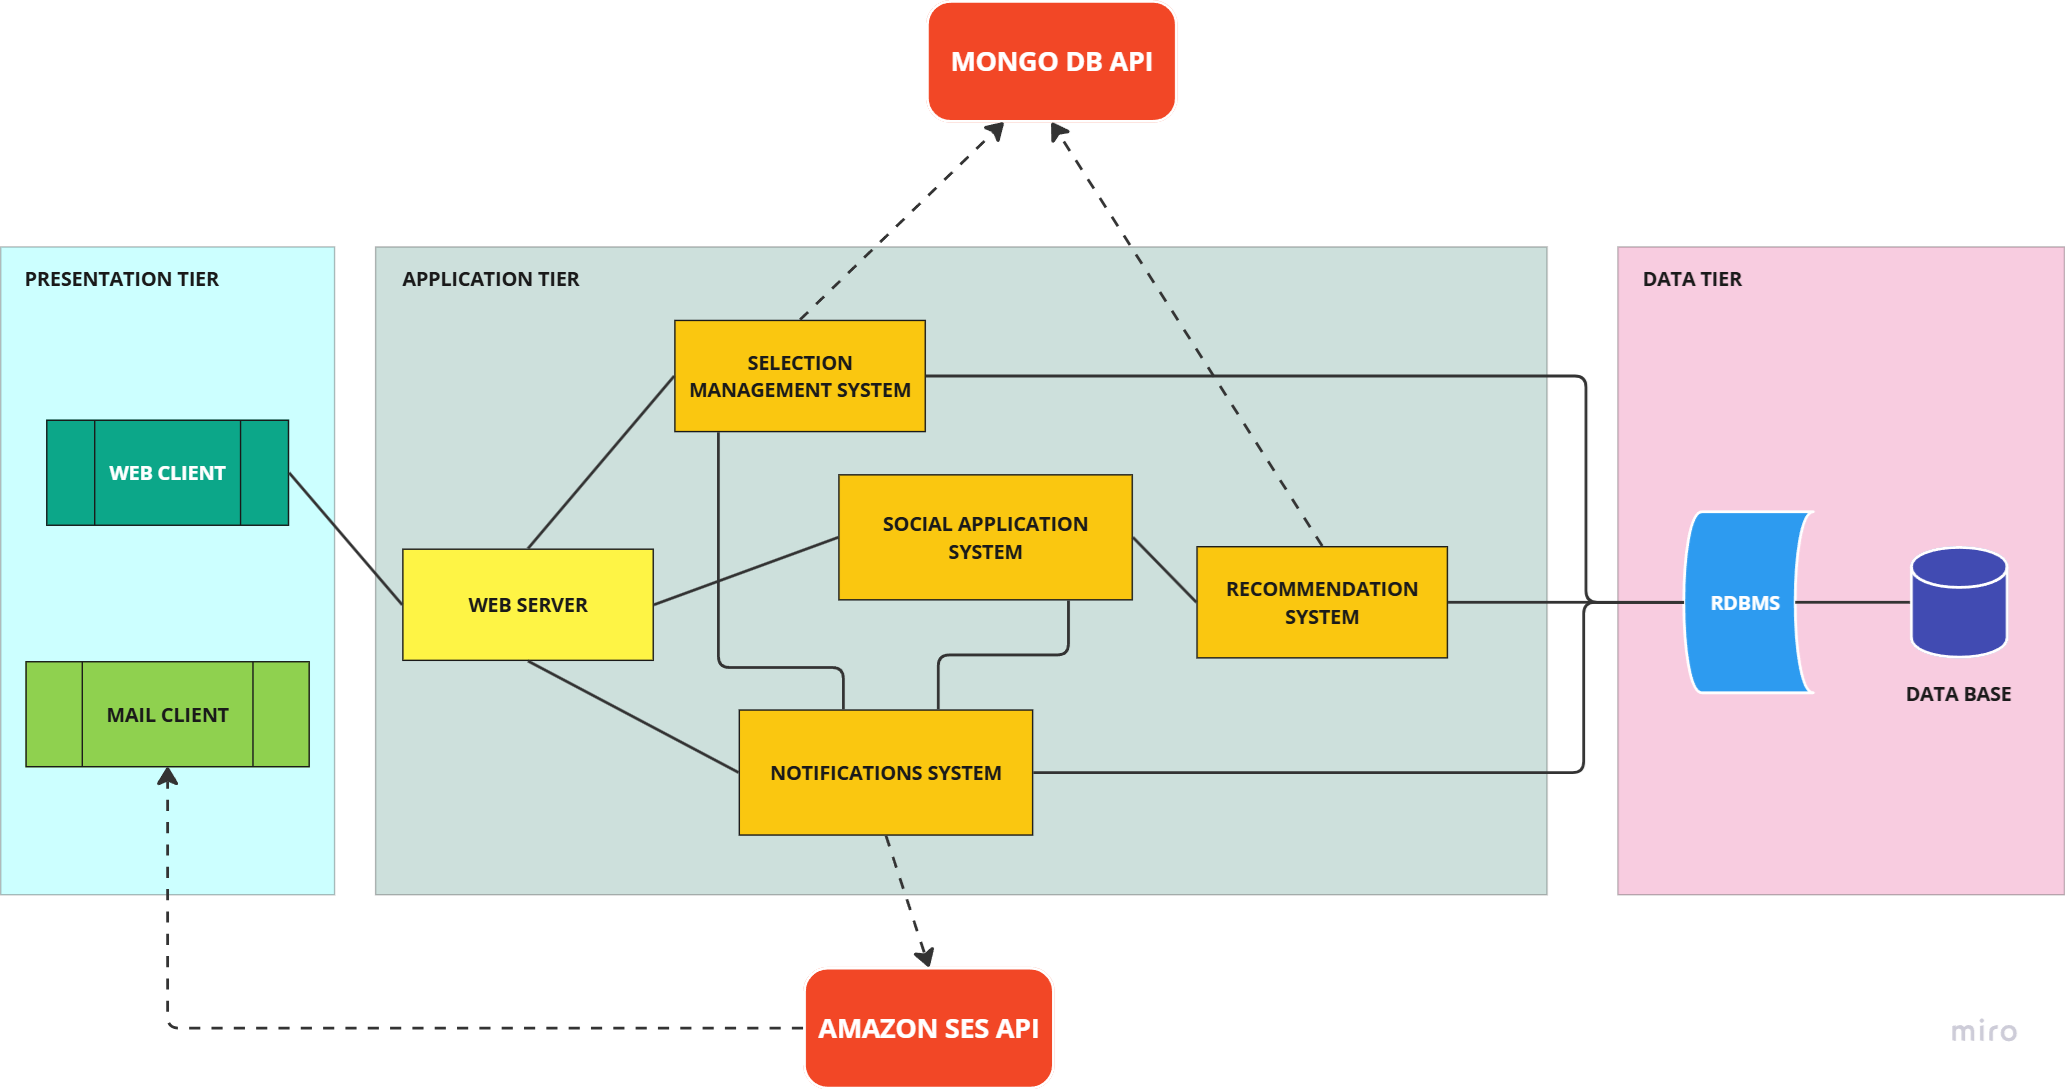
\includegraphics{informalArc.png}
	
	\section{Deployment View}
	\section{Runtime View}
		\begin{figure}[H]
			\centering
			{\bfseries [UC1] - Student Registration}
			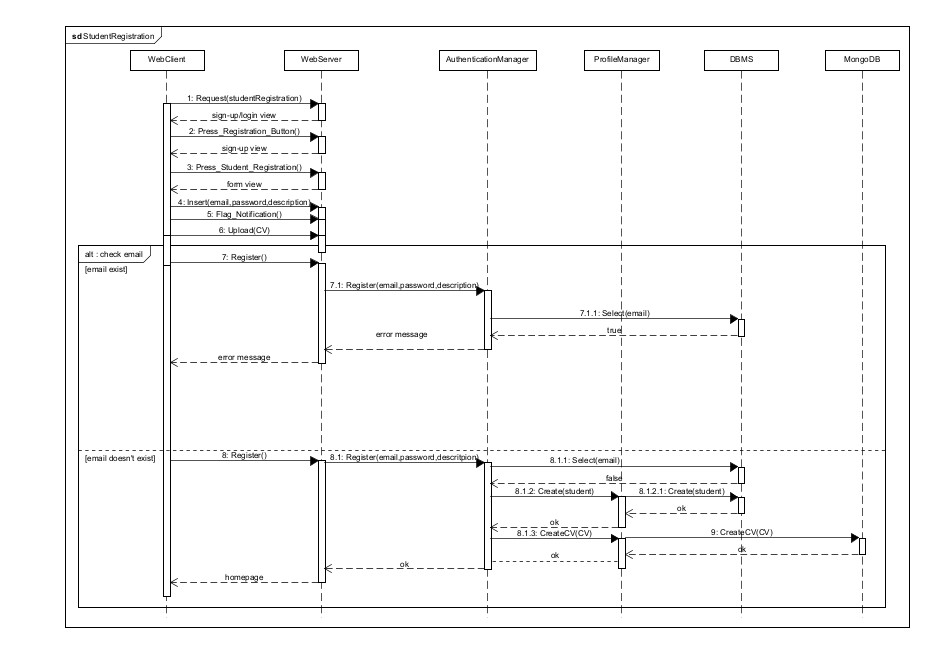
\includegraphics[scale=0.3]{StudentRegistrationDD.jpg}
			\caption{[UC1] - Student Registration}
		\end{figure}
			
		The figure shows the student registration process; the request is sent to Authentication Manager, which is also responsible for receiving the registration form completed by the student. Once received, Authentication Manager queries the DBMS to check if the student's email is already present in the database. If it is not present, the student will be saved in the database, while the CV will be stored in MongoDB as an unstructured data. If the email is already in the database, an error message will be displayed to the student.
		
		\begin{figure}[H]
			\centering
			{\bfseries [UC2] - Company Registration}
			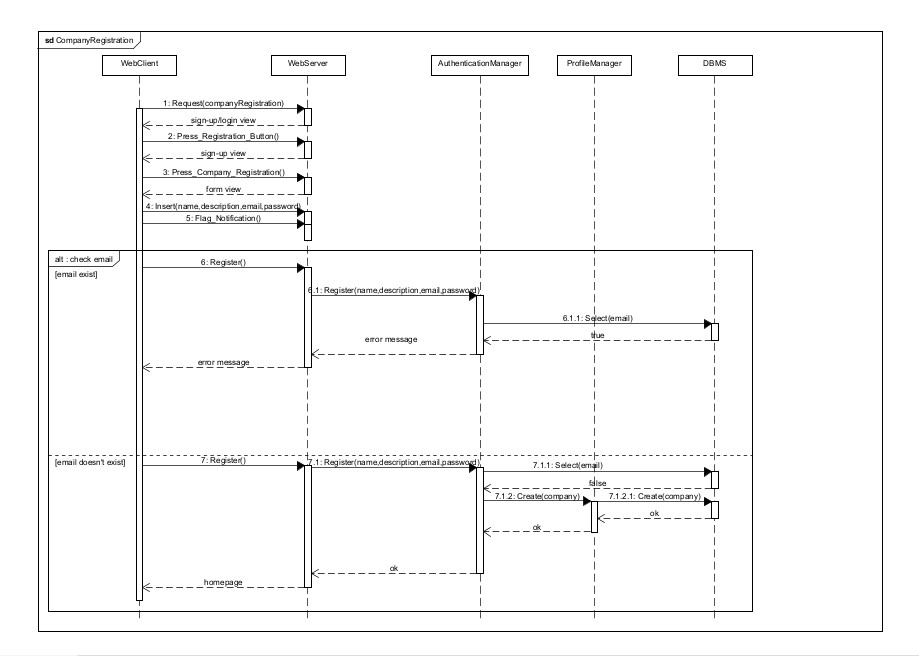
\includegraphics[scale=0.3]{CompanyRegistrationDD.jpg}
			\caption{[UC2] - Company Registration}
		\end{figure}
		
		The figure shows the company registration process; the flow is similar to the student registration case, with the difference that in this case, different data is saved (the company has a name and a description), and all the data is stored in the relational database since they are all structured data.
		
		\begin{figure}[H]
			\centering
			{\bfseries [UC3] - User Login}
			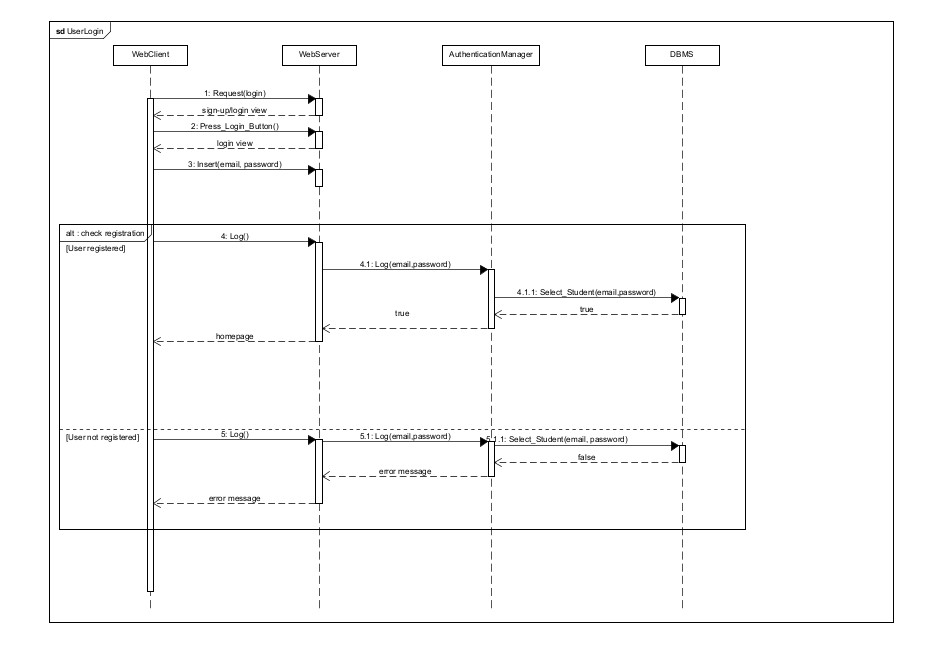
\includegraphics[scale=0.3]{UserLoginDD.jpg}
			\caption{[UC3] - User Login}
		\end{figure}
		
		The figure shows the user login process, which is similar for both students and companies; in this case, the request is handled by the Authentication Manager, which selects the student from the database to allow login. If the student is not found, an error message is displayed.
		
		
		\begin{figure}[H]
			\centering
			{\bfseries [UC4] - Publish Internship Advice}
			\caption{[UC4] - Publish Internship Advice}
			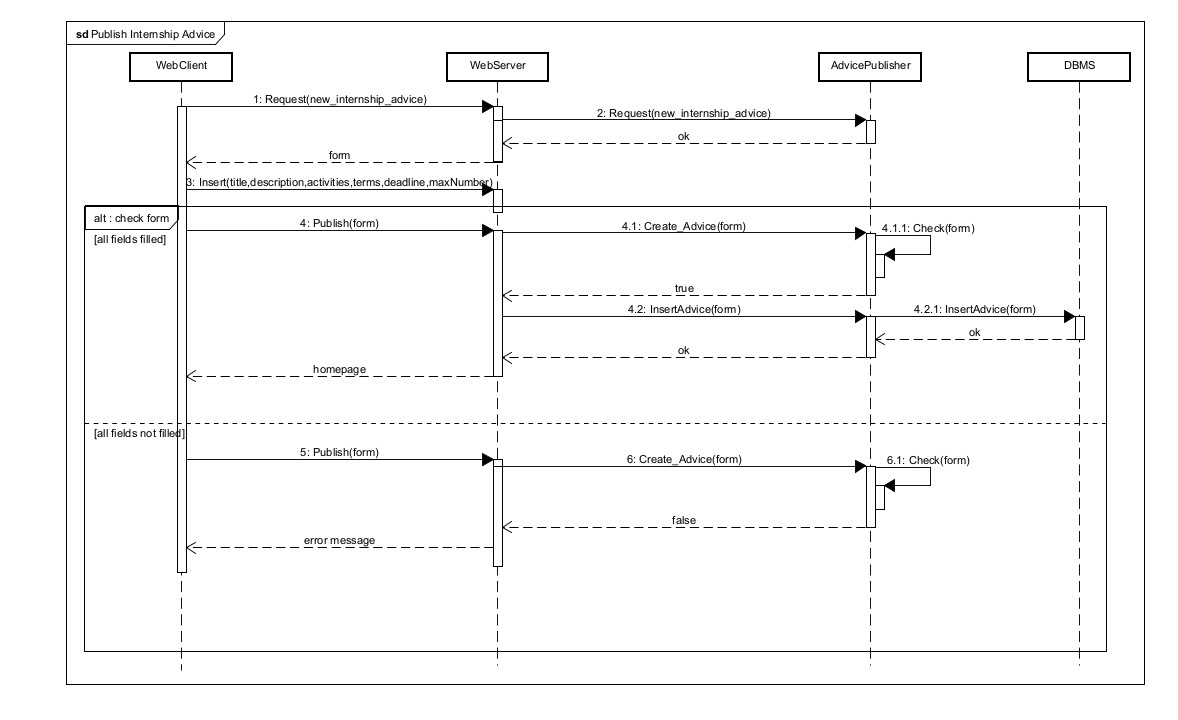
\includegraphics[scale=0.3]{PublishInternshipAdviceDD.jpg}
			
		\end{figure}
		
		the figure shows the publish internship advice process; the web server redirect the request to the publisher advice component, which create a new advice and put it in the relational DB; before that, the publisher advice check if the form is already filled: in the negative case, it presents to the client an error message.
		
		
		\begin{figure}[H]
			\centering
			{\bfseries [UC5] - Search of all Internships}
			\caption{[UC5] - Search of all Internships}
			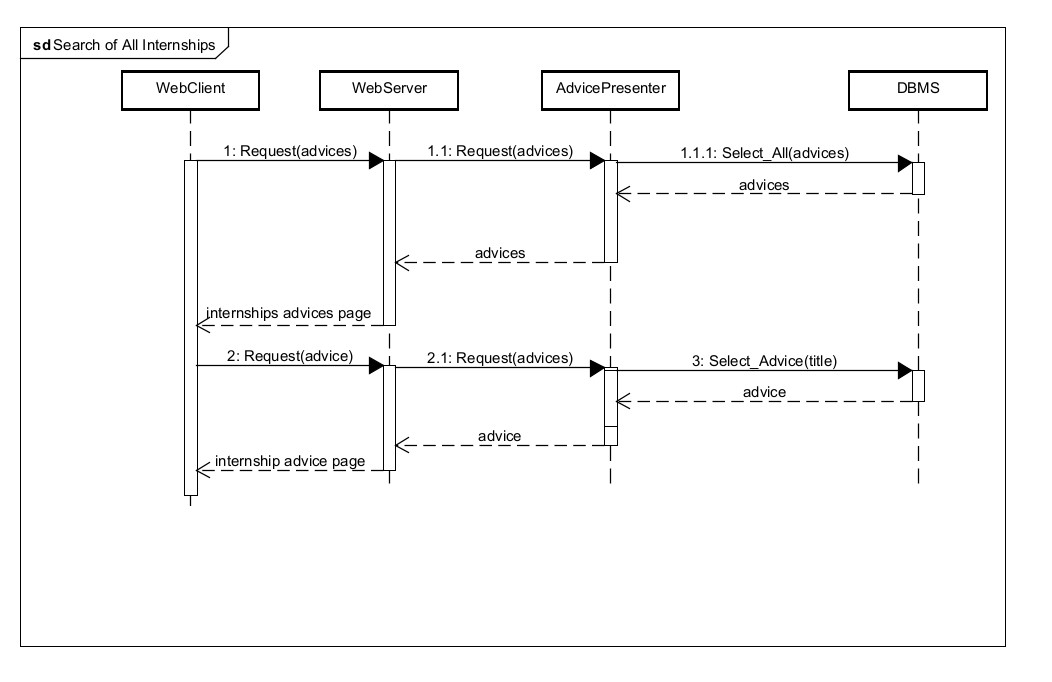
\includegraphics[scale=0.3]{SearchAllInternshipsDD.jpg}
			
		\end{figure}
		
		
		the figure shows the process of search on all the internships: the web server sends the request to the advice presenter, which selects all the advice from the relational DB; then the client requests a specific advice and the flow is the same: the advice presenter is called and it selects the advice (by title) from the relational DB
		
		\begin{figure}[H]
			\centering
			{\bfseries [UC6] - Search of All Companies}
			\caption{[UC6] - Search of All Companies}
			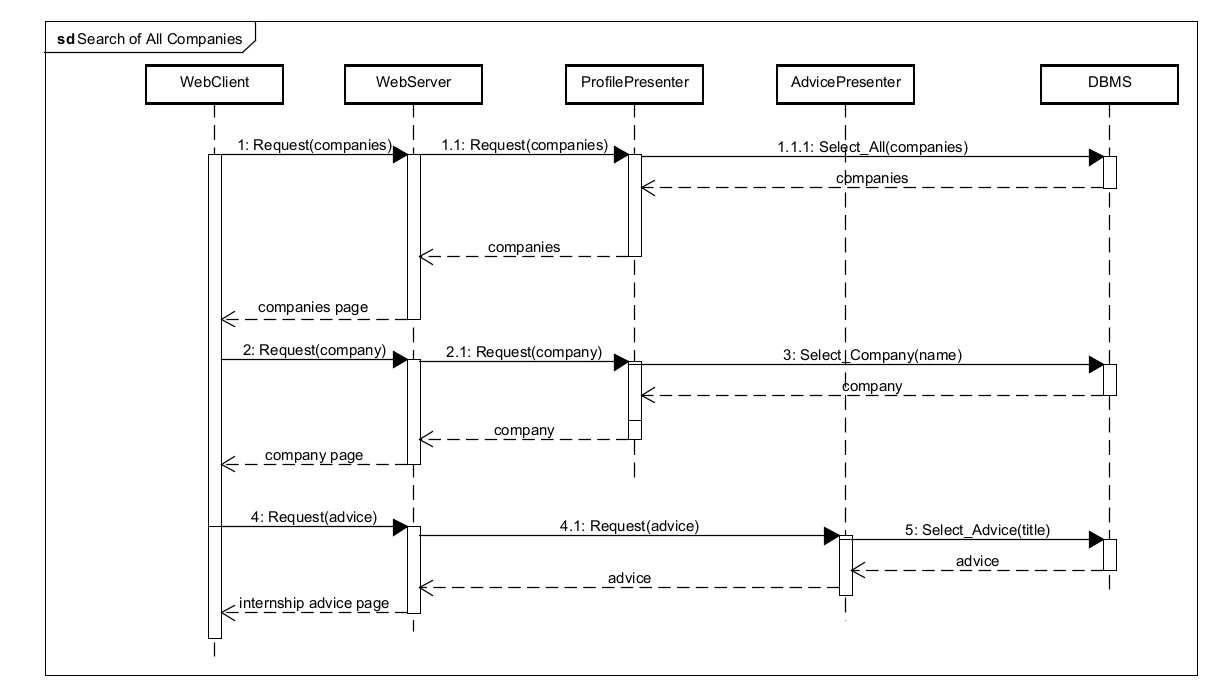
\includegraphics[scale=0.3]{SearchAllCompaniesDD.jpg}
			
		\end{figure}
		
		
		the figure shows the process of search on all the companies: the web server sends the request to the profile presenter, which selects all the companies from the relational DB; then the client requests a specific advice: the advice presenter is called and it selects the advice (by title) from the relational DB and it is presented to the client
		
		\begin{figure}[H]
			\centering
			{\bfseries [UC7] - Search an Internship by Name}
			\caption{[UC7] - Search an Internship by Name}
			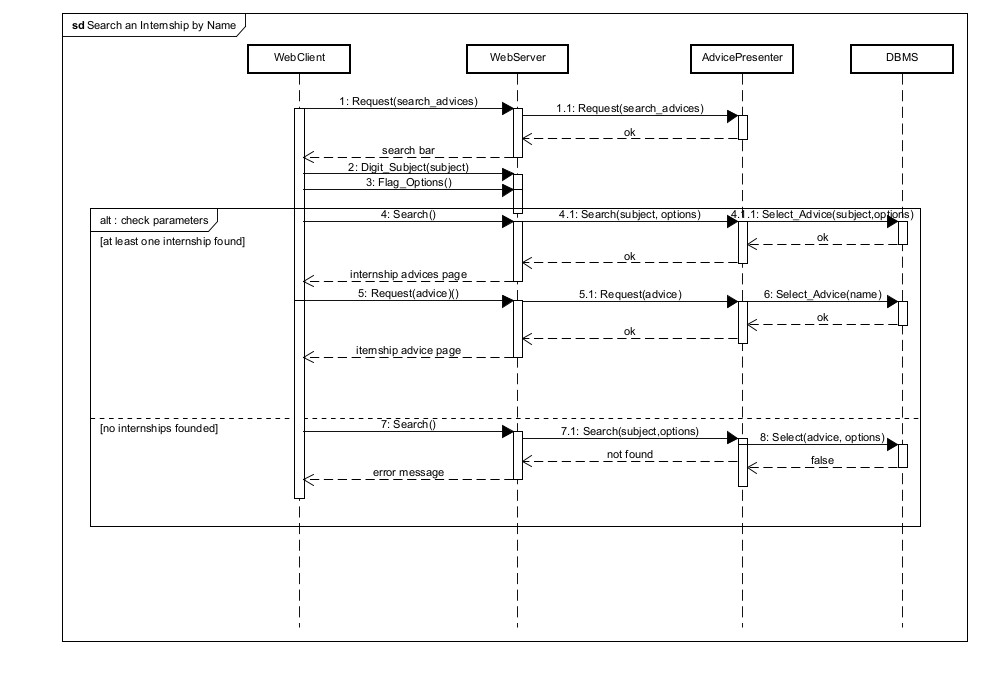
\includegraphics[scale=0.3]{SearchByNameDD.jpg}
			
		\end{figure}
		
		the figure shows the process of proactive search of an internship; the request is redirect to the advice presenter, which receive then from the client the subject searched and the options flag; then this component query the relational DB to find if exists at least one advice that match the subject and the option: if it is true, return the list of this advice and then the client requests a specific one (as we mentioned before); if it is false, return an error message.
		
		
		\begin{figure}[H]
			\centering
			{\bfseries [UC8] - Internship Recommendation}
			\caption{[UC8] - Internship Recommendation}
			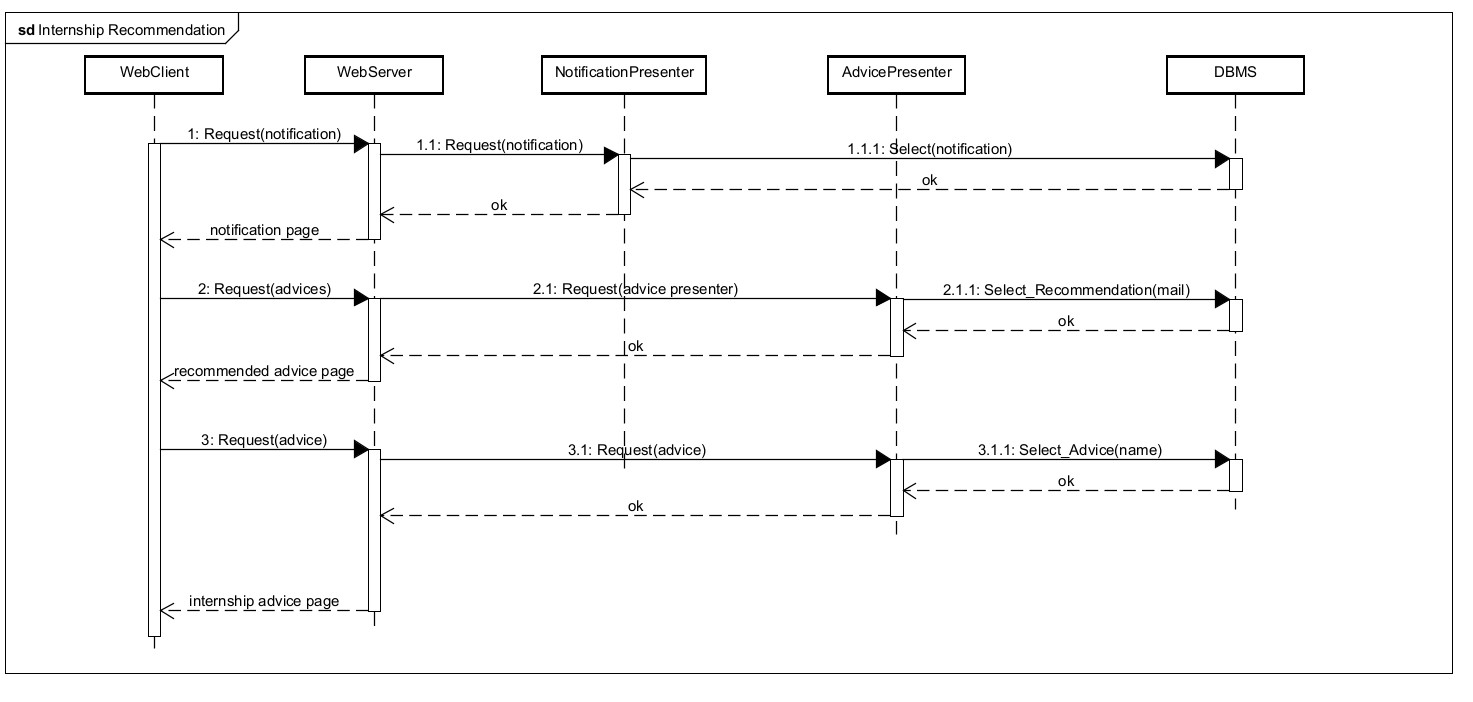
\includegraphics[scale=0.3]{InternshipRecommendationDD.jpg}
			
		\end{figure}
		
		the figure shows how the students can look for internships advice recommended; first of all, the client displays a notification: the web server sends the notification to the notification presenter, which retrieves it from the database. Subsequently, to view the recommended advice, the web server forwards the request to the advice presenter, which retrieves the recommended advice related to the student from the database and then presents it to the client. Finally, the client selects an advice in the manner described earlier.
		
		
		\begin{figure}[H]
			\centering
			{\bfseries [UC9] - Students Recommendation}
			\caption{[UC9] - Students Recommendation}
			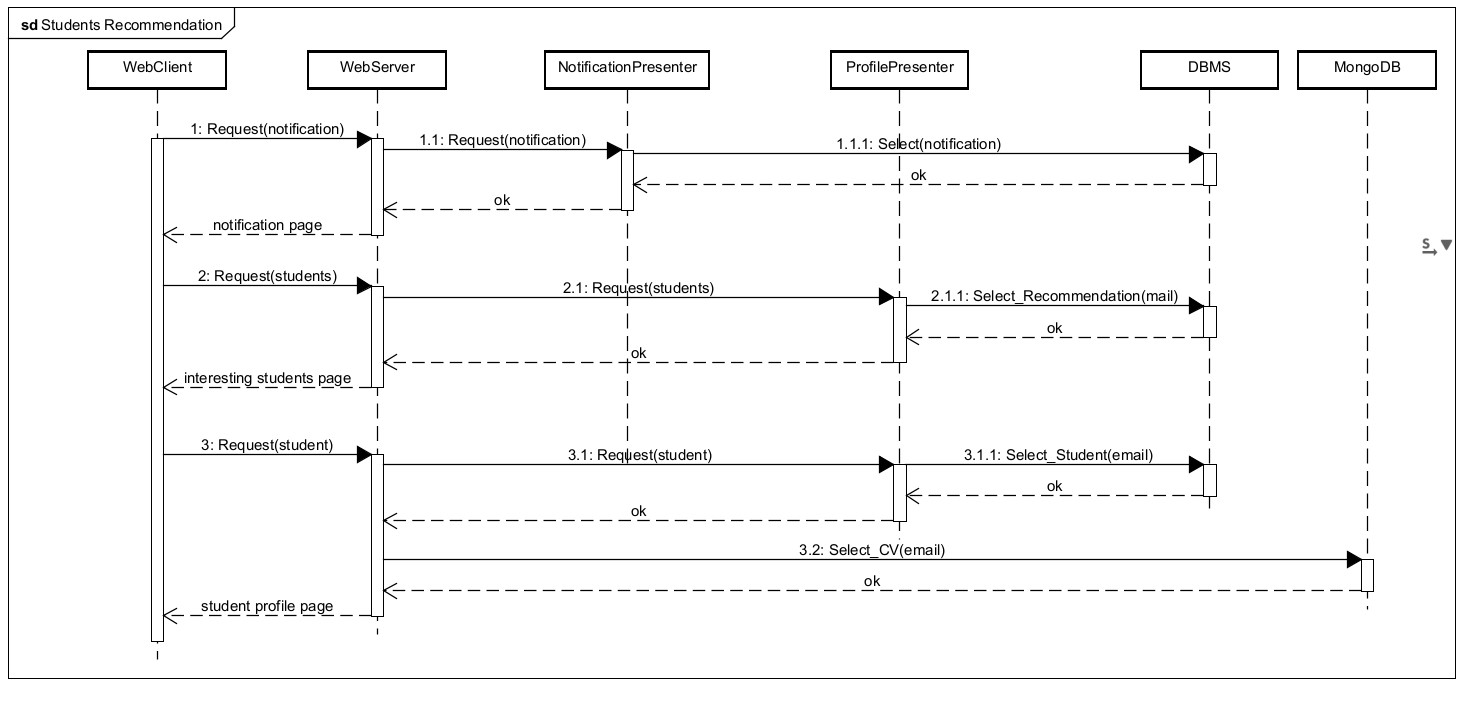
\includegraphics[scale=0.3]{StudentsRecommendationDD.jpg}
			
		\end{figure}
		
		the figure shows how the companies can look for students recommended; first of all, the client displays a notification: the web server sends the notification to the notification presenter, which retrieves it from the database. Subsequently, to view the recommended students, the web server forwards the request to the profile presenter, which retrieves the recommended students related to the company from the database and then presents it to the client. Finally, the client selects a students(note that it has to retrieve also the CV from MongoDB, instead the other data are retrieved from the relational DB)
		
		\begin{figure}[H]
			\centering
			{\bfseries [UC10-a] - Student Application Process-send application}
			\caption{[UC10-a] - Student Application Process-send application}
			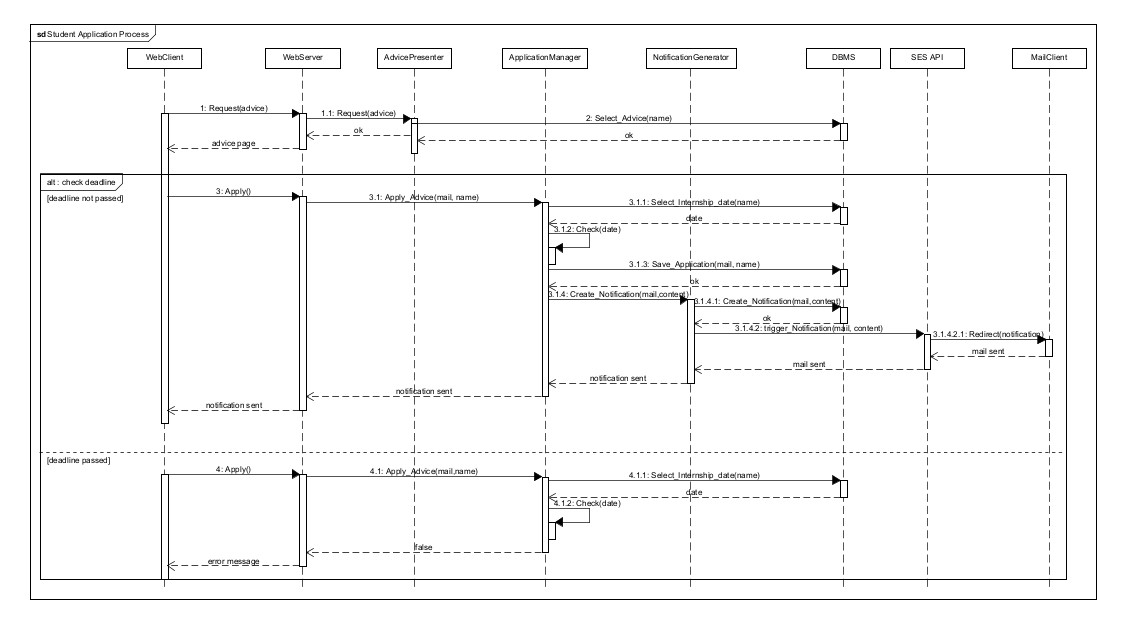
\includegraphics[scale=0.3]{StudentApplicationProcess1DD.jpg}
			
		\end{figure}
		
		\begin{figure}[H]
			\centering
			{\bfseries [UC10-b] - Student Application Process-accept application}
			\caption{[UC10-b] - Student Application Process-accept application}
			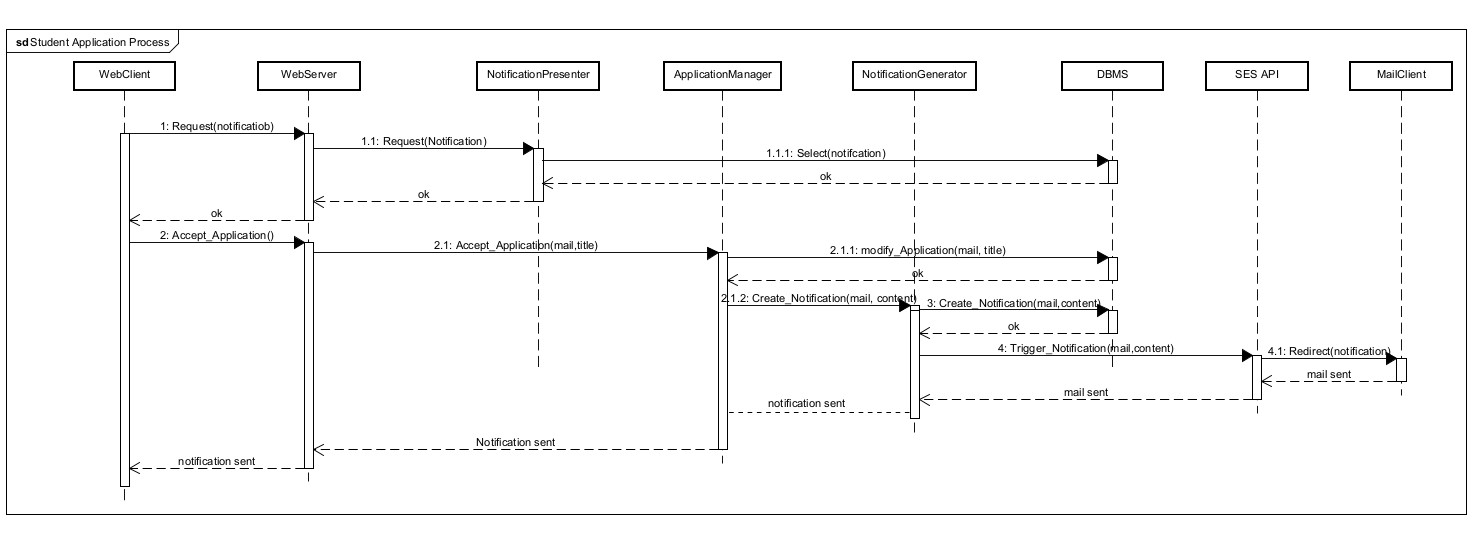
\includegraphics[scale=0.3]{StudentApplicationProcess2DD.jpg}
			
		\end{figure}
		
		In these two sequence diagrams, the entire student application process is depicted. Both the application submission phase and the acceptance of an application utilize the Application Manager component, which is responsible for inserting the newly created application into the relational database. The Notification Generator component then triggers the email sending process and sends a notification to the recipient company, which accepts the application by sending a response notification (Figure 2). It should be noted that the company can also reject the application, but the modeling is identical to the acceptance process.
		
		
		
		\begin{figure}[H]
			\centering
			{\bfseries [UC11-a] - Company Send of Proposal-send proposal}
			\caption{[UC11-a] - Company Send of Proposal - send proposal}
			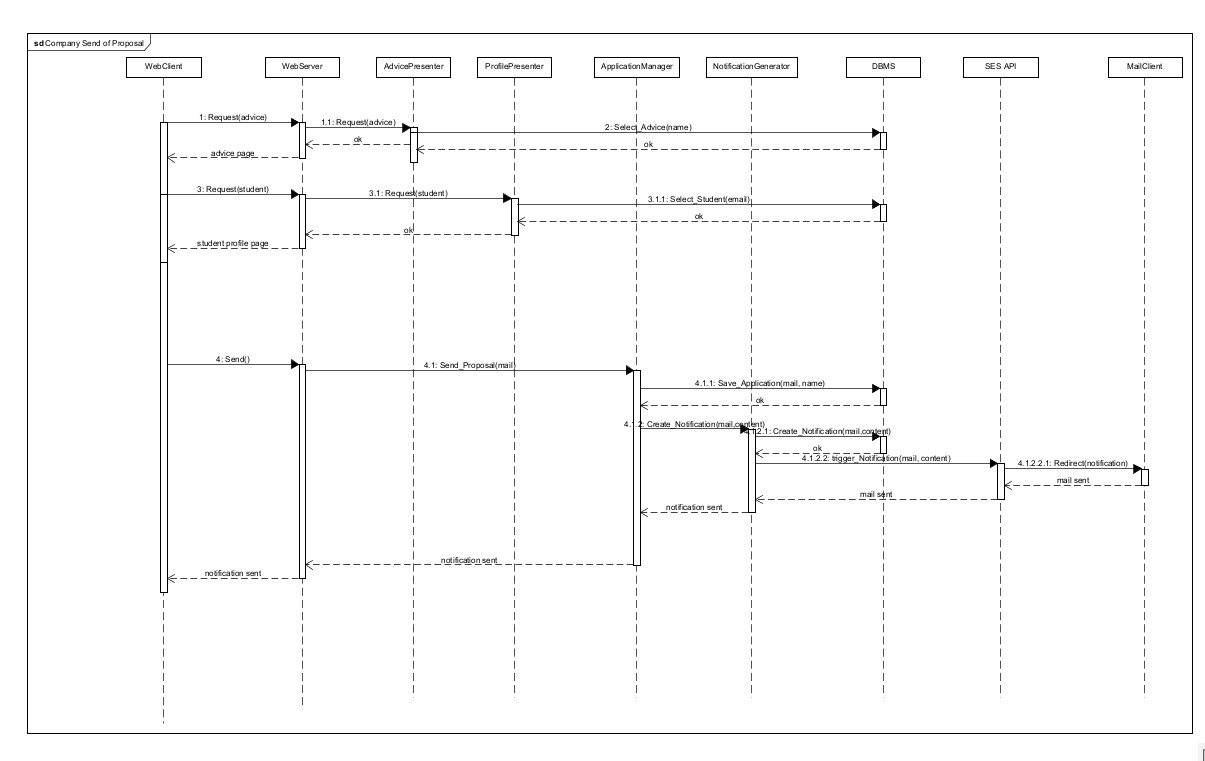
\includegraphics[scale=0.3]{SendProposal1DD.jpg}
			
		\end{figure}
		
			\begin{figure}[H]
			\centering
			{\bfseries [UC11-b] - Company Send of Proposal-accept proposal}
			\caption{[UC11-b] - Company Send of Proposal - accept proposal}
			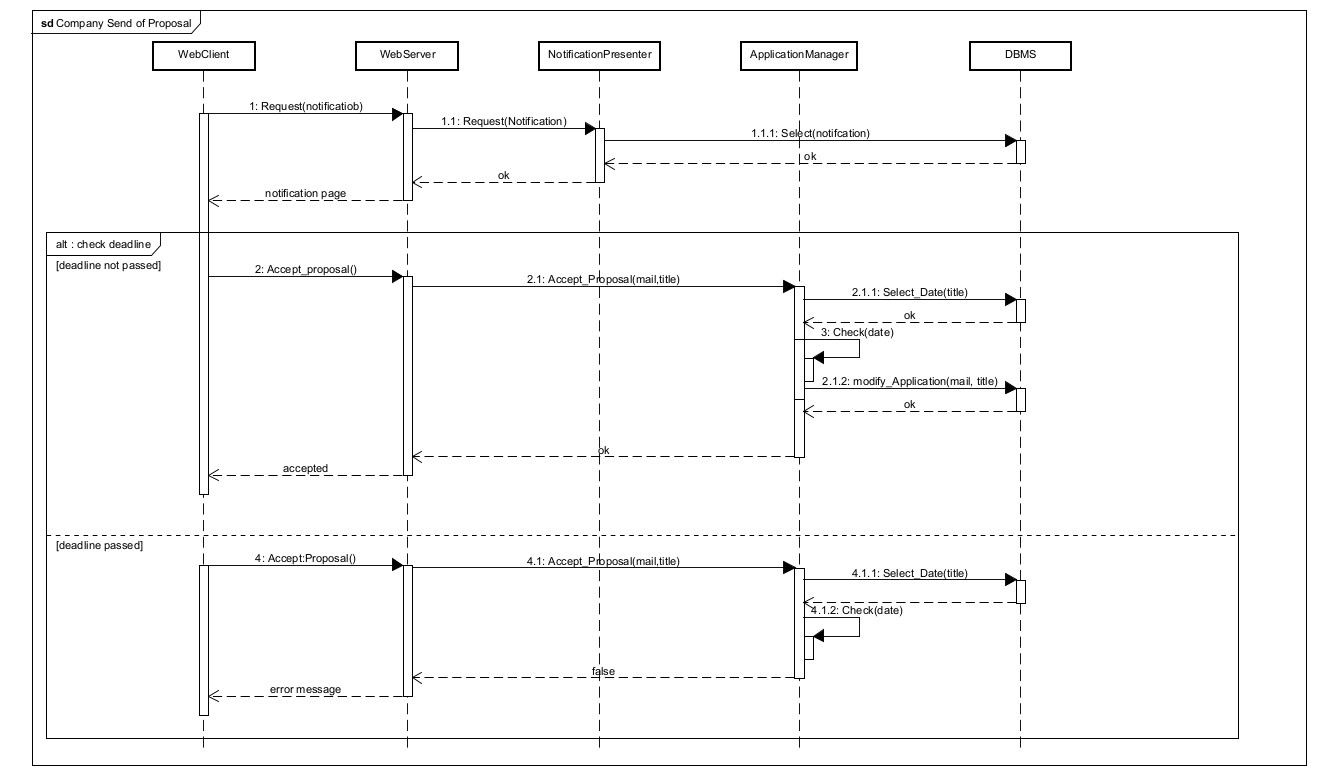
\includegraphics[scale=0.3]{SendProposal2DD.jpg}
			
		\end{figure}
		
		
		
		The two sequence diagrams show the entire process of submitting a proposal by a company. In both figures, it is the Application Manager component that handles the creation of a new application, sending the notification (with email trigger), and managing the acceptance. The acceptance can only occur if the deadline has not yet passed; otherwise, an error message is displayed.
		
		
		
		
		
		
		
		\begin{figure}[H]
			\centering
			{\bfseries [UC12] - Selection Process Configuration}
			\caption{[UC12] - Selection Process Configuration}
			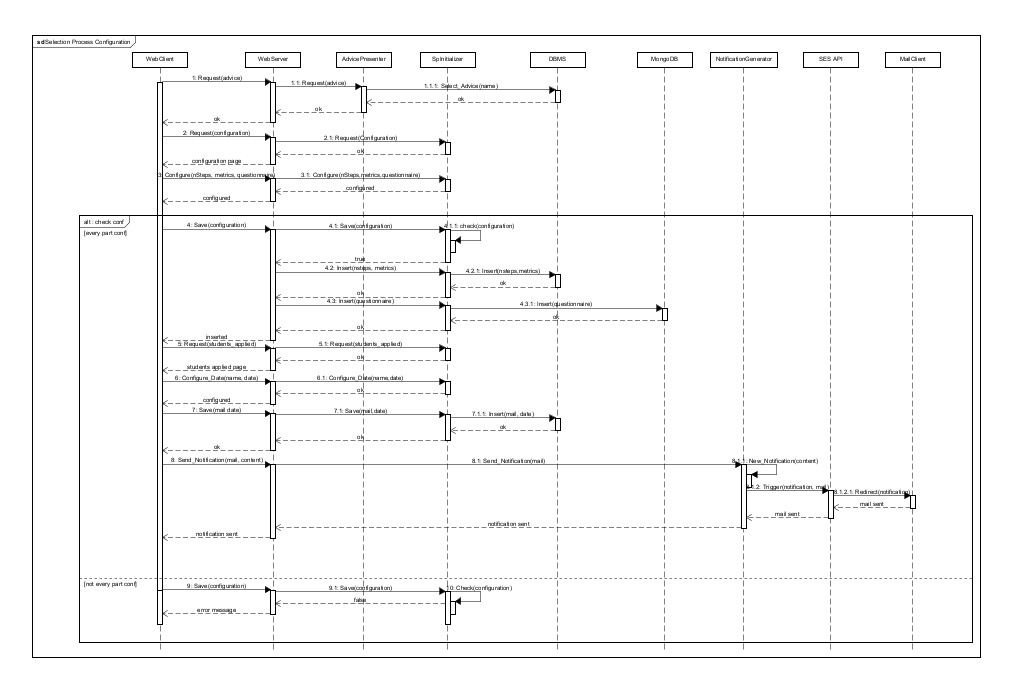
\includegraphics[scale=0.3]{ProcessConfigurationDD.jpg}
			
		\end{figure}
		
		
		the figure shows the selection process configuration; initially, the client requests the advice it wants to view (and the advice presenter retrieves it from the database). Subsequently, to initialize the selection process, a request is sent to the SP initializer, which displays the configuration to be completed. The client completes the configuration by entering the number of steps, metrics, and defining the questionnaires for the questions. The configuration is then saved by the SP initializer in the databases: metrics and the number of steps are stored in the relational database, while the questionnaires are saved in MongoDB’s non-relational database (as they are unstructured data).
		
		Afterward, similarly, the interview dates for each student are defined and saved in the relational database. Finally, the client sends a notification: the Notification Generator handles generating the notification, then triggers the SES API, which directs the email to the student's Mail client. If the configuration is incomplete, an error message will be displayed to the client.
		
		
		\begin{figure}[H]
			\centering
			{\bfseries [UC14] - Collection of Student Selection Process Feedback}
			\caption{[UC14] - Collection of Student Selection Process Feedback}
			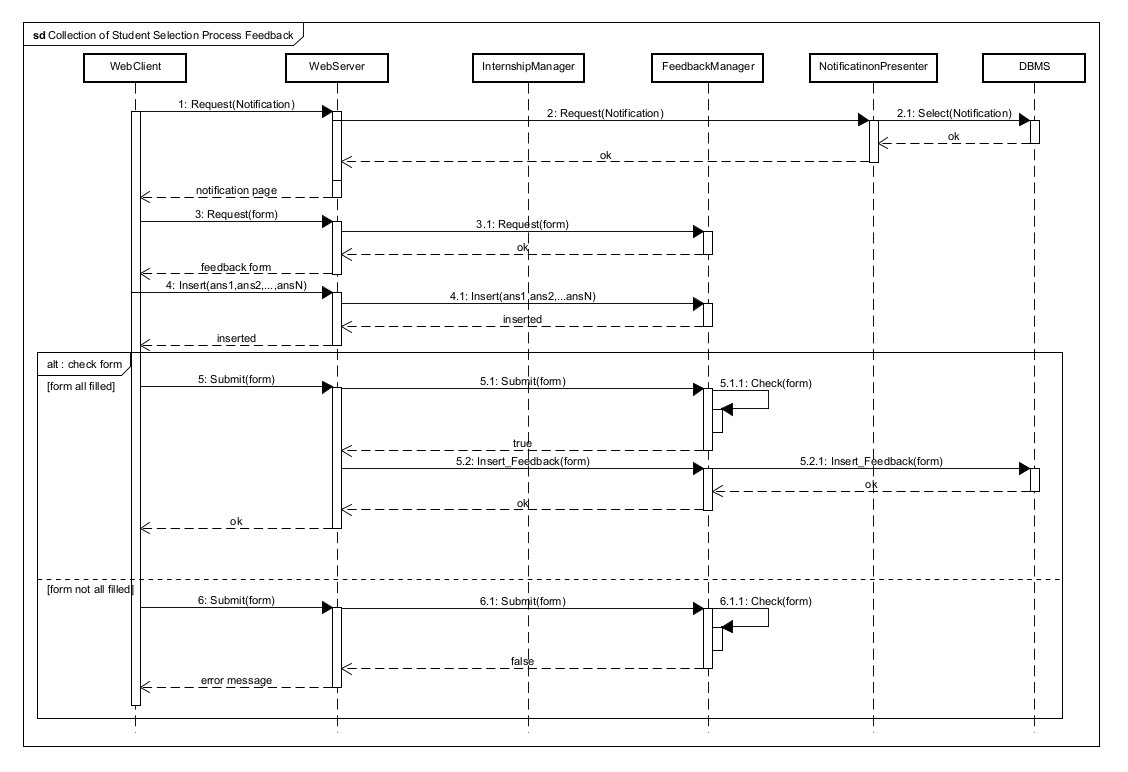
\includegraphics[scale=0.3]{StudentFeedbackDD.jpg}
		\end{figure}
		
		the figure shows the collection of students selection process feedback; the client requests the notification containing the form to be filled out to provide feedback (the form is displayed by the Feedback Manager). The client fills out the form and submits it to the Feedback Manager, which handles querying the database to insert the feedback. If the form is incomplete, the Feedback Manager will display an error message to the client.
		
		
		\begin{figure}[H]
			\centering
			{\bfseries [UC15] - Collection of Company Selection Process Feedback}
			\caption{[UC15] - Collection of Company Selection Process Feedback}
			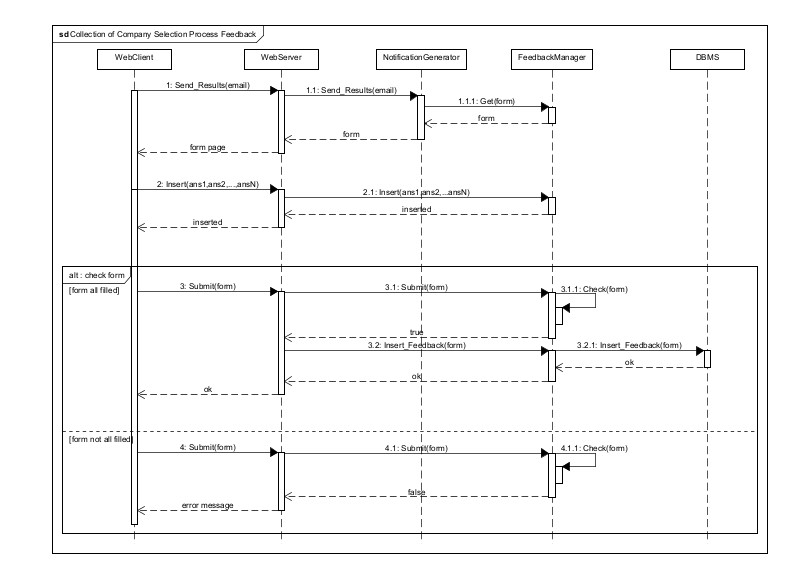
\includegraphics[scale=0.3]{CompanyFeedbackDD.jpg}
			
		\end{figure}
		
		
		the figure shows the collection of company selection process feedback; after sending the result notification, the client obtain the form from the Feedback Manager. The client fills out the form and submits it to the Feedback Manager, which handles querying the database to insert the feedback. If the form is incomplete, the Feedback Manager will display an error message to the client.
		
		
		\begin{figure}[H]
			\centering
			{\bfseries [UC16] - Collection of Internships Feedback}
			\caption{[UC16] - Collection of Internships Feedback}
			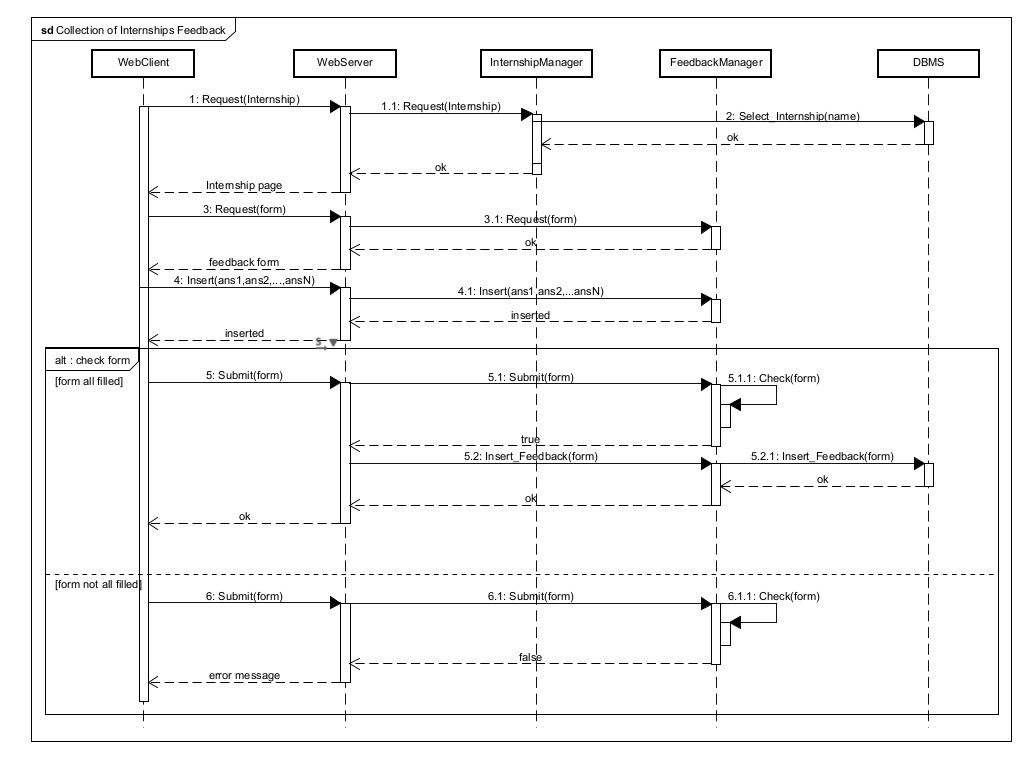
\includegraphics[scale=0.3]{InternshipFeedbackDD.jpg}
			
		\end{figure}
		
		the figure shows the collection of Internships feedback; the client requests an internship they want to view (in this case, an ongoing internship), which is displayed by the Internship Manager. Subsequently, the client requests the form to provide feedback, shown by the Feedback Manager. The client then fills out the form, and the Feedback Manager saves the results in the relational database, provided the form is fully completed. Otherwise, the Feedback Manager shows an error message to the client.
		
		
		
		
		\begin{figure}[H]
			\centering
			{\bfseries [UC17] - Collection of Complaints}
			\caption{[UC17] - Collection of Complaints}
			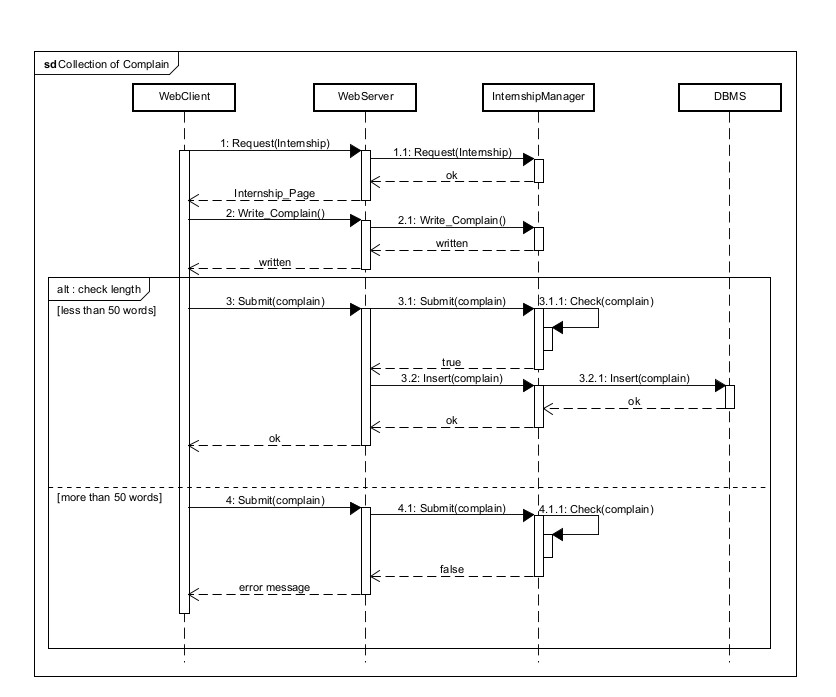
\includegraphics[scale=0.3]{CollectionComplaintsDD.jpg}
			
		\end{figure}
		
		the figure shows the collection of complaints written by the user; he flow is similar to the one described for the collection of internship feedback, with the difference that, in this case, the Feedback Manager performs a check on the length of the complaint (which must be less than 50 words).
		
		
		\begin{figure}[H]
			\centering
			{\bfseries [UC18] - Ongoing internship closing}
			\caption{[UC18] - Ongoing internship closing}
			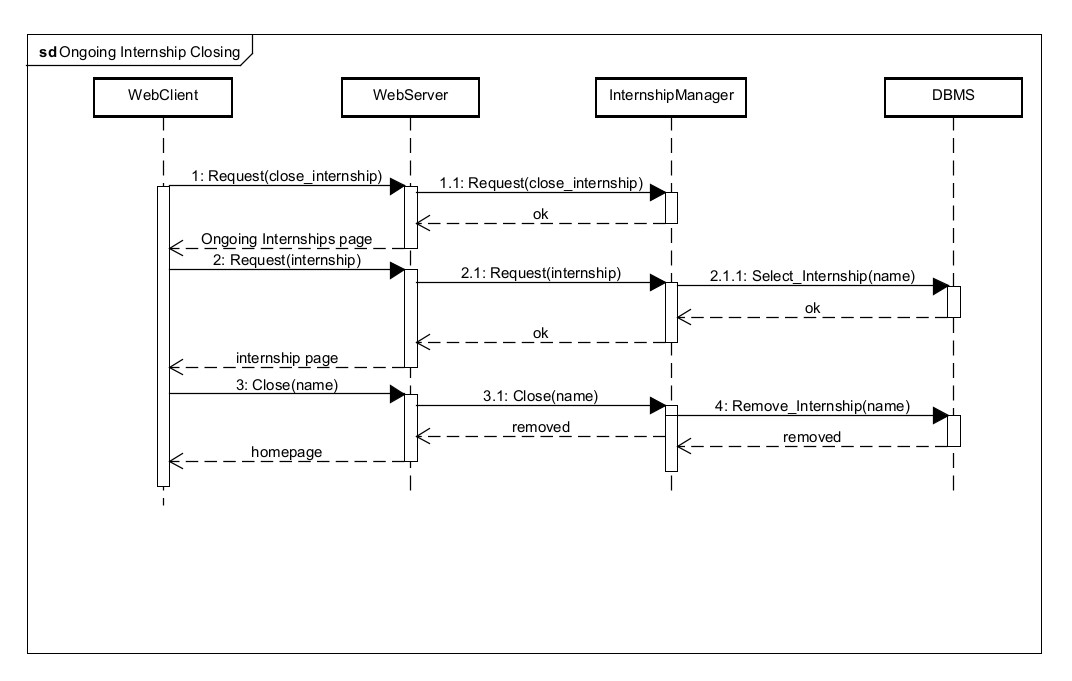
\includegraphics[scale=0.3]{DeleteDD.jpg}
			
		\end{figure}
		
		
		The figure shows the process of closing an internship when it is completed. The Client, when requesting to close an internship, invokes the Internship Manager component, which is responsible for removing the internship from the relational database.
		
		
		
		
	\section{Component Interfaces}
	
	\textbf{Authentication Manager}
	\begin{itemize}
		\item Register(email,password,description)
		\item Register(name, description,email,password)
		\item Login(email,password)
	\end{itemize}
	
	\textbf{Application Manager}
	\begin{itemize}
		\item Apply\_Advice(mail,name)
		\item Send\_Proposal(mail)
		\item Accept\_Application(mail,title)
		\item Accept\_Proposal(mail,title)
	\end{itemize}
	
	\textbf{Advice Presenter}
	\begin{itemize}
		\item Request(advices)
		\item Request(search\_advices)
		\item Search(subject, options)
		\item Request(advice)
		\item Request(notification)
	\end{itemize}
	
	\textbf{Advice Publisher}
	\begin{itemize}
		\item Request(new\_internship\_advice)
		\item Create\_Advice(form)
		\item insert\_Advice(form)
		
	\end{itemize}
	
	\textbf{Feedback Manager}
	\begin{itemize}
		\item Request(form)
		\item Insert(ans1,ans2,..., ansN)
		\item Submit(form)
		\item Insert\_Feedback(form)
	\end{itemize}
	
	\textbf{Internship Manager}
	\begin{itemize}
		\item Request(internship)
		\item Write\_Complaint()
		\item Submit(complain)
		\item Insert(complain)
		\item Request(close\_internship)
		\item Close(name)
	\end{itemize}
	
	\textbf{Profile Manager}
	\begin{itemize}
		\item Create(student)
		\item Create\_CV(CV)
		\item Create(company)
	\end{itemize}
	
	\textbf{Profile Presenter}
	\begin{itemize}
		\item Request(companies)
		\item Request(company)
		\item Request(students)
		\item Request(student)
	\end{itemize}
	
	\textbf{Recommendation Interface}
	\textbf{Recommendation Analyzer}
	\textbf{Recommendation Presenter}
	
	\textbf{Notification Presenter}
	\begin{itemize}
		\item Request(notification)
	\end{itemize}
	
	\textbf{Notification Generator}
	\begin{itemize}
		\item Create\_Notification(mail, content)
		
	\end{itemize}
	
	\textbf{SP Initiallizer}
	\begin{itemize}
		\item Request(configuration)
		\item Confgiure(nSteps, metrics, questionnaire)
		\item Save(configuration)
		\item Insert(nSteps, metrics)
		\item Insert(questionnaire)
		\item Request(student\_applied)
		\item Configure\_Date(email,date)
		\item Save(mail, date)
	\end{itemize}
	
	\textbf{SP Presenter}
	\begin{itemize}
		\item Request(date)
		\item Request(results)
	\end{itemize}
	
	\textbf{SES API}
	\begin{itemize}
		\item Trigger\_Notification(mail,content)
	\end{itemize}
	
	\textbf{Mail\_Client}
	\begin{itemize}
		\item Redirect(notification)
	\end{itemize}
	
	\textbf{DBMS}
	\begin{itemize}
		\item Select(email)
		\item Create(student)
		\item Create(company)
		\item Select\_Student(email,password)
		\item Insert\_Advice(form)
		\item Select\_All(advices)
		\item Select\_Advice(title)
		\item Select\_Advice(subject,options)
		\item Select(notification)
		\item Select\_Recommendation(mail)
		\item Select\_Internship\_Date(mail)
		\item Save\_Application(mail,name)
		\item Create\_Notification(mail,content)
		\item Modify\_Application(mail,title)
		\item Insert(nStesp,metrics)
		\item Insert(mail,date)
		\item Insert\_Feedback(form)
		\item Insert(complain)
		\item Select\_Internship(name)
		\item Remove\_Internship(name)
	\end{itemize}
	
	\textbf{MongoDB}
	\begin{itemize}
		\item CreateCV(CV)
		\item Select\_CV(email)
		\item Insert(questionnaire)
	\end{itemize}













	\section{Data Logic Model}
		Starting from the high-level class diagram presented in the RASD, the logic scheme of the database is designed:
		\begin{figure}[H]
			\centering
			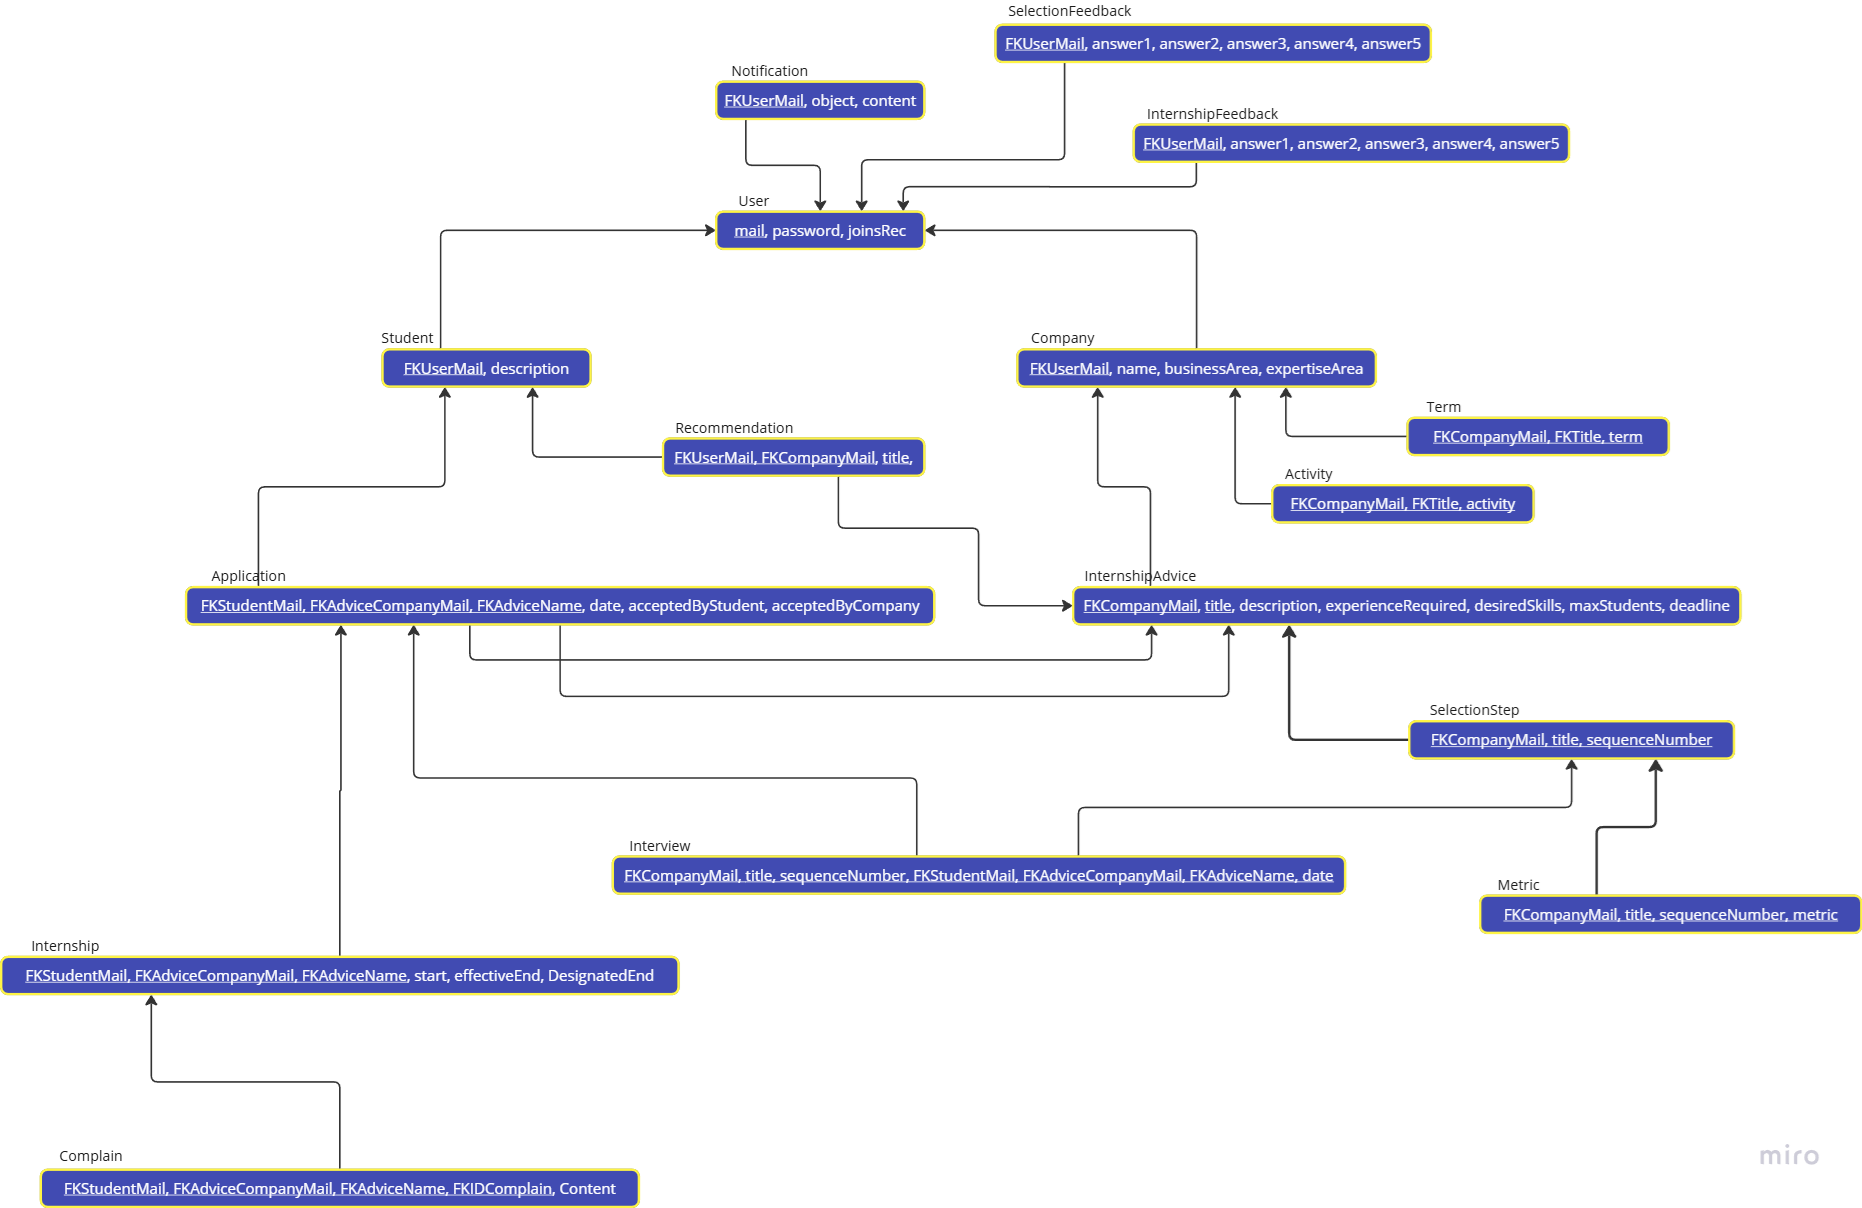
\includegraphics{datalogic.png}
			\caption{Data logic model scheme}
		\end{figure}
		Classes are almost one-to-one mapped with tables (with reification of vector attributes), the only relevant differences are:
		\begin{itemize}
			\item feedback-tables has an attribute for each questionnaire answer, this is not a concern since questionnaires are static (each questionnaire always has the same set of questions);
			\item the \emph{Recommendation} table was added, in order to store the recommendation analysis results;
			\item selection process questionnaires and CVs are missing since they are stored in Mongo DB (they are far more suitable for an unstructured data representation).
		\end{itemize}
	\section{Selected Architectural Styles and Patterns}
	
		\subsection{3-tier architecture}
			As mentioned in section 2.1, the architecture used for the system implementation is a 3-tier architecture, which offers significant advantages in terms of modularity and scalability. Regarding the data layer, a relational database was chosen to manage structured data, while a non-relational database was adopted to handle unstructured data more flexibly, such as CVs and questionnaires with the responses from the selection process.
			
			
		\subsection{Model-View-Controller(MVC) pattern}
			As previously mentioned, S\&C was designed to be developed as a web application. Consequently, one of the most commonly used patterns for building this type of application is the MVC pattern. This pattern divides the application into three main components:
			
			\begin{itemize}
				\item \textbf{Model}: Manages the data, business logic, and rules of the application. It acts as the interface between the database and the rest of the application.
				\item \textbf{View}: Handles the presentation layer, defining how the data is displayed to the user.
				\item \textbf{Controller}: Serves as an intermediary between the Model and the View, processing user inputs, updating the Model, and determining which View to display.
				
				
			\end{itemize}
			
			he use of this pattern once again provides significant advantages in terms of modularity and separation of concerns. Additionally, it enhances the reliability of the developed system and promotes reusability. Finally, having a clear separation between the Model, View, and Controller makes it much easier to perform functional testing of the system.
		
		\subsection{Other Design Decisions}
			
			
			
			
			
			
			
			
			
			
			